\NeedsTeXFormat{LaTeX2e}
%
%\documentclass[aps,pra,showpacs,amsmath,amssymb,superscriptaddress,nofootinbib]{revtex4}
\documentclass[]{article}
\usepackage{graphicx}% Include figure files
% \usepackage{bm}% bold math
% \usepackage{amssymb}
% \usepackage{amsmath}
% \usepackage{latexsym}
% \usepackage{color}
% \usepackage{soul}
% \usepackage{nopageno}
% \usepackage{tikz}
%%

\begin{document}  

\thispagestyle{empty}

% figure created using https://www.mathcha.io/editor#

%%%%%%%%%%%%%%%%%%%%%%%%%%%%%%%%  put here figure %%%%%%%%%%%%%%%%%%%%%%%%%%%%%%%%%%%%%%%%%%%%%%%%
% \tikzset{every picture/.style={line width=0.75pt}} %set default line width to 0.75pt        



\begin{figure}
% \label{fig:8keV}
% \caption{Numerical evaluation of diffracted intensity by a \SI{250}{\micro\meter} thick Si 111 symmetric Laue crystal calculated using equation~(\ref{eq:Dhpropagated}) for a bent (R~= \SI{1}{\meter}) crystal and $p$~= \SI{50}{\meter}. 
% a) on-axis intensity for a photon energy of 8.3 keV. 
% Inset: transverse profile at the focal distances (maximum values):  
% $q_1$~= \SI{651}{\milli\meter} (blue), and
% $q_2$~= \SI{1330}{\milli\meter} (green).
% b) on-axis intensity for a photon energy of 17 keV.
% Inset: transverse profile at the focal distances (maximum values):
% $q_1$~= \SI{625}{\milli\meter} (blue), and 
% $q_2$~= \SI{1372}{\milli\meter} (green).

% }
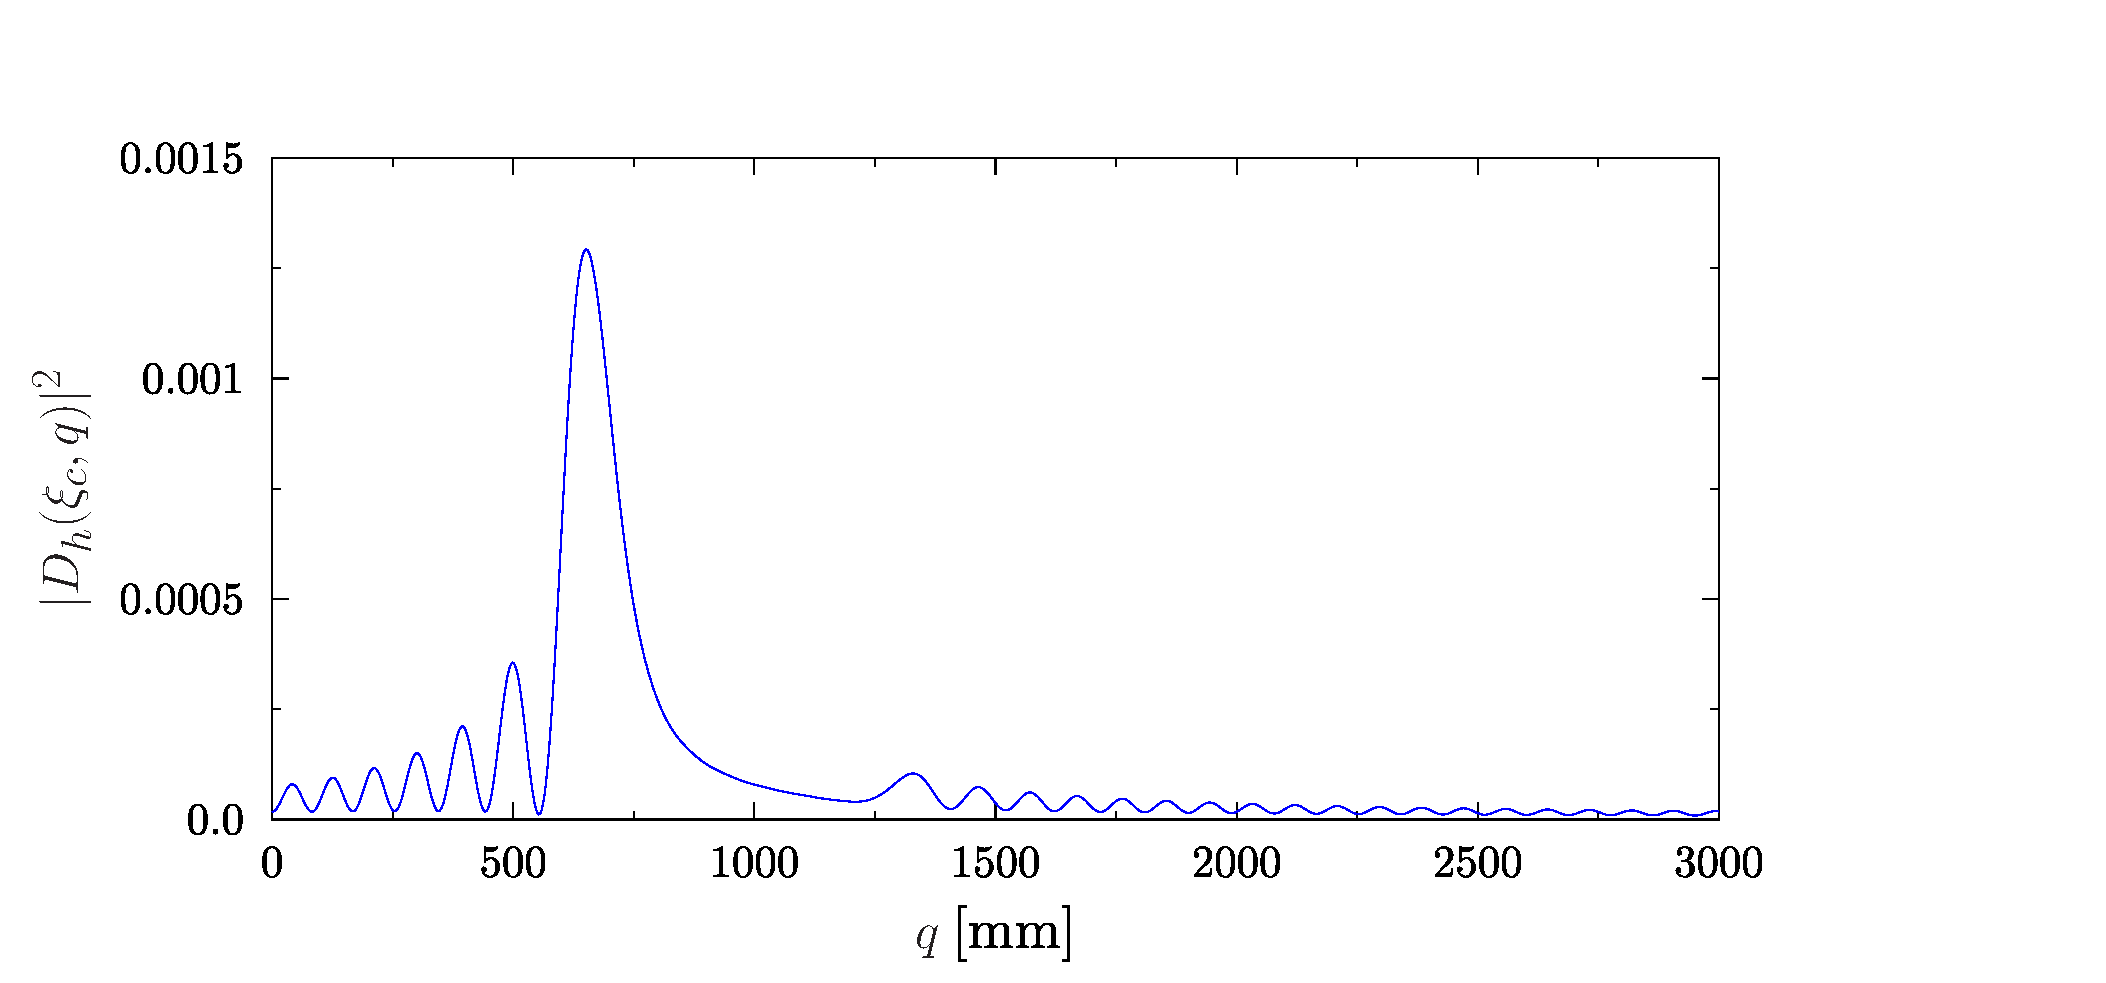
\includegraphics[width=1\textwidth]{bent1m8keV.eps}

\begin{picture}(0,0)
\setlength{\unitlength}{1cm}
\put(4.5,2){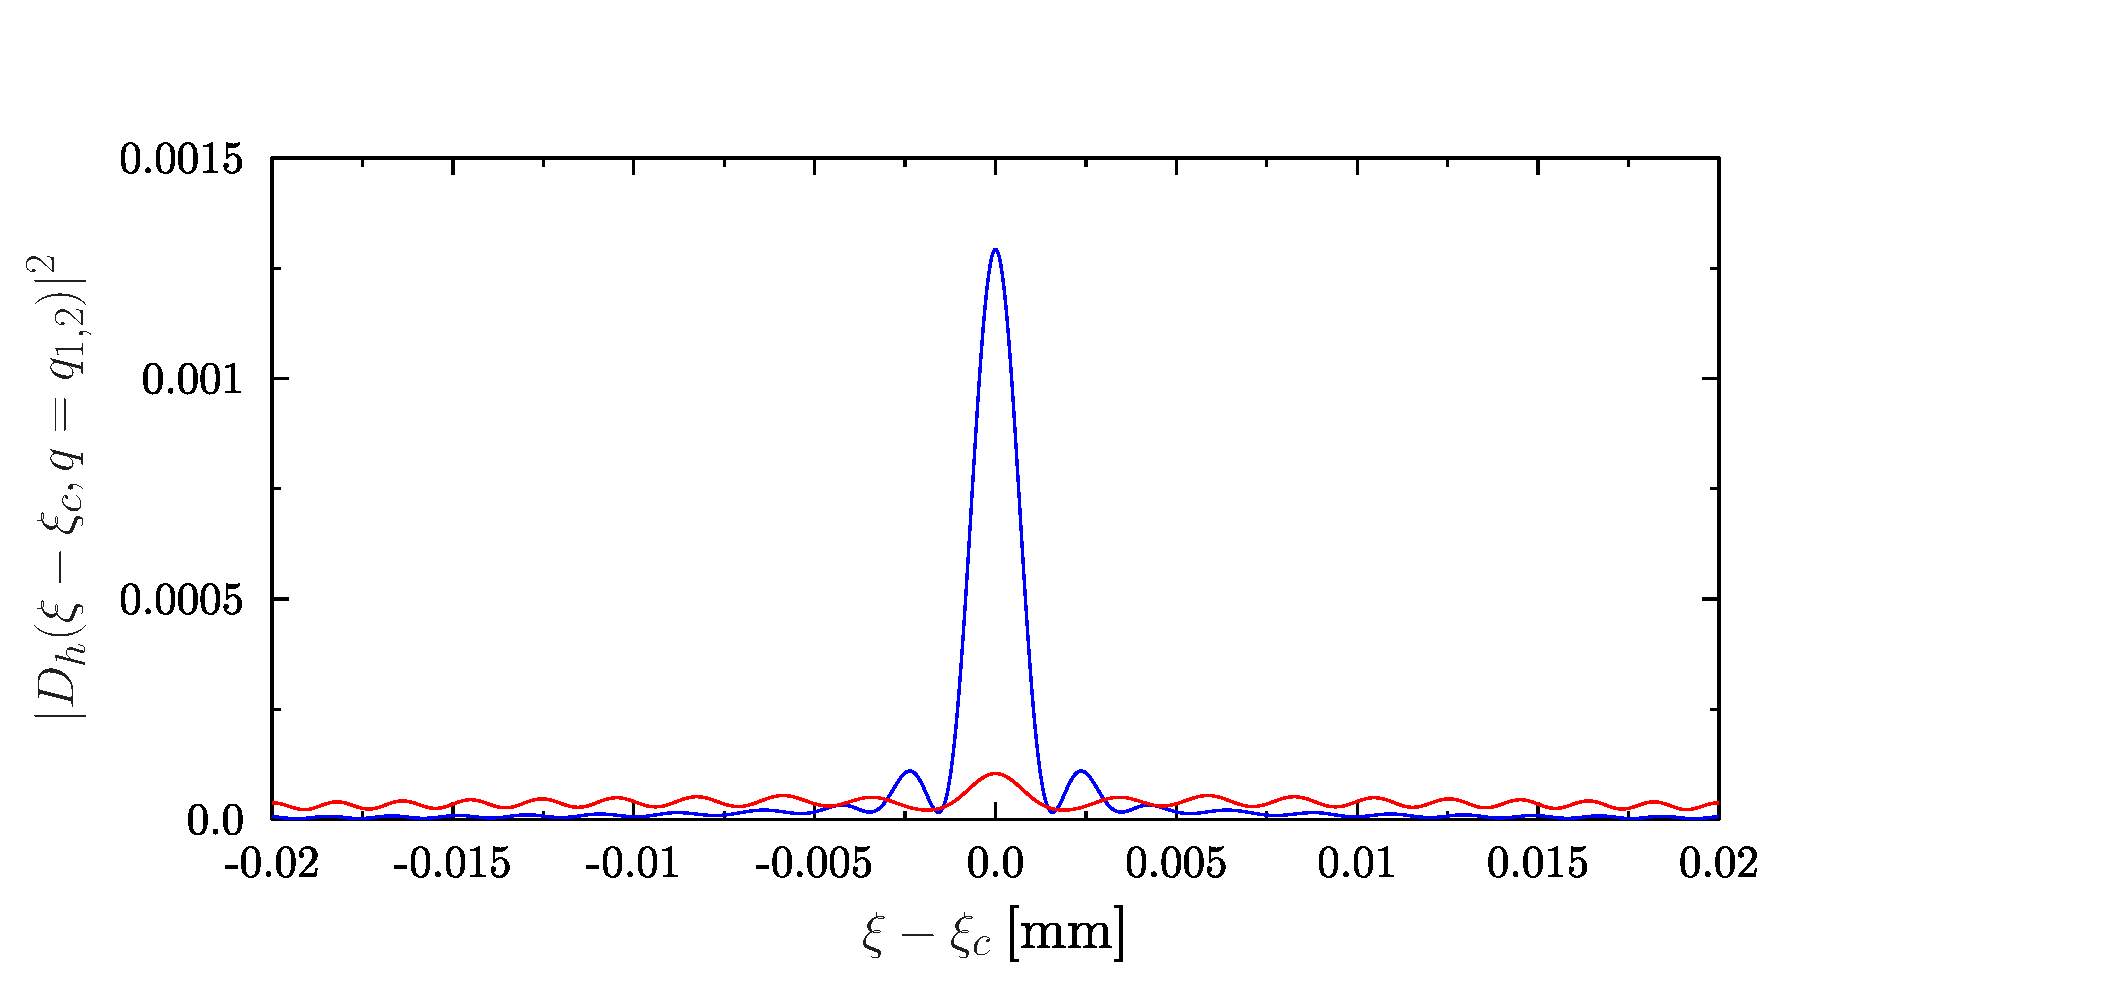
\includegraphics[width=0.5\textwidth]{bent1m8keV_profile.eps}}
\end{picture}

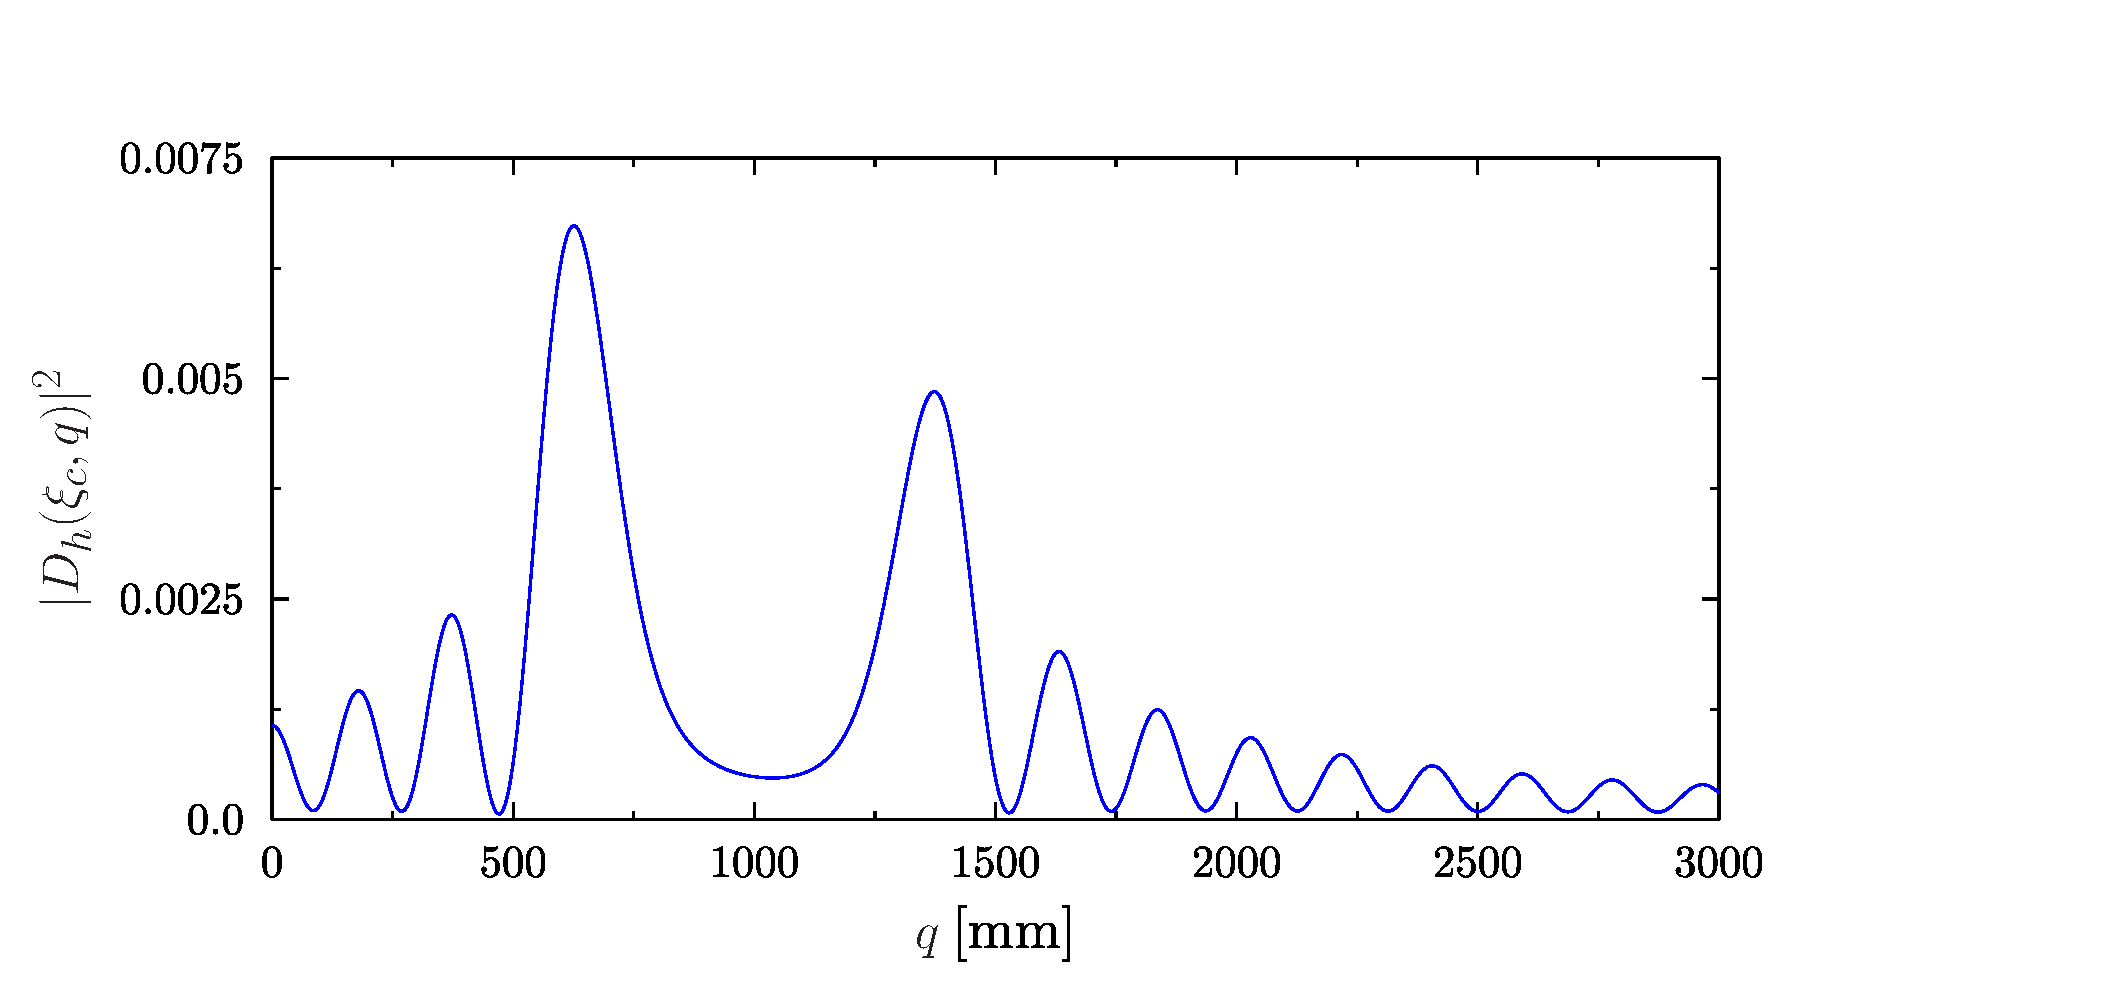
\includegraphics[width=1\textwidth]{bent1m17keV.eps}

\begin{picture}(0,0)
\setlength{\unitlength}{1cm}
\put(5.25,2.8){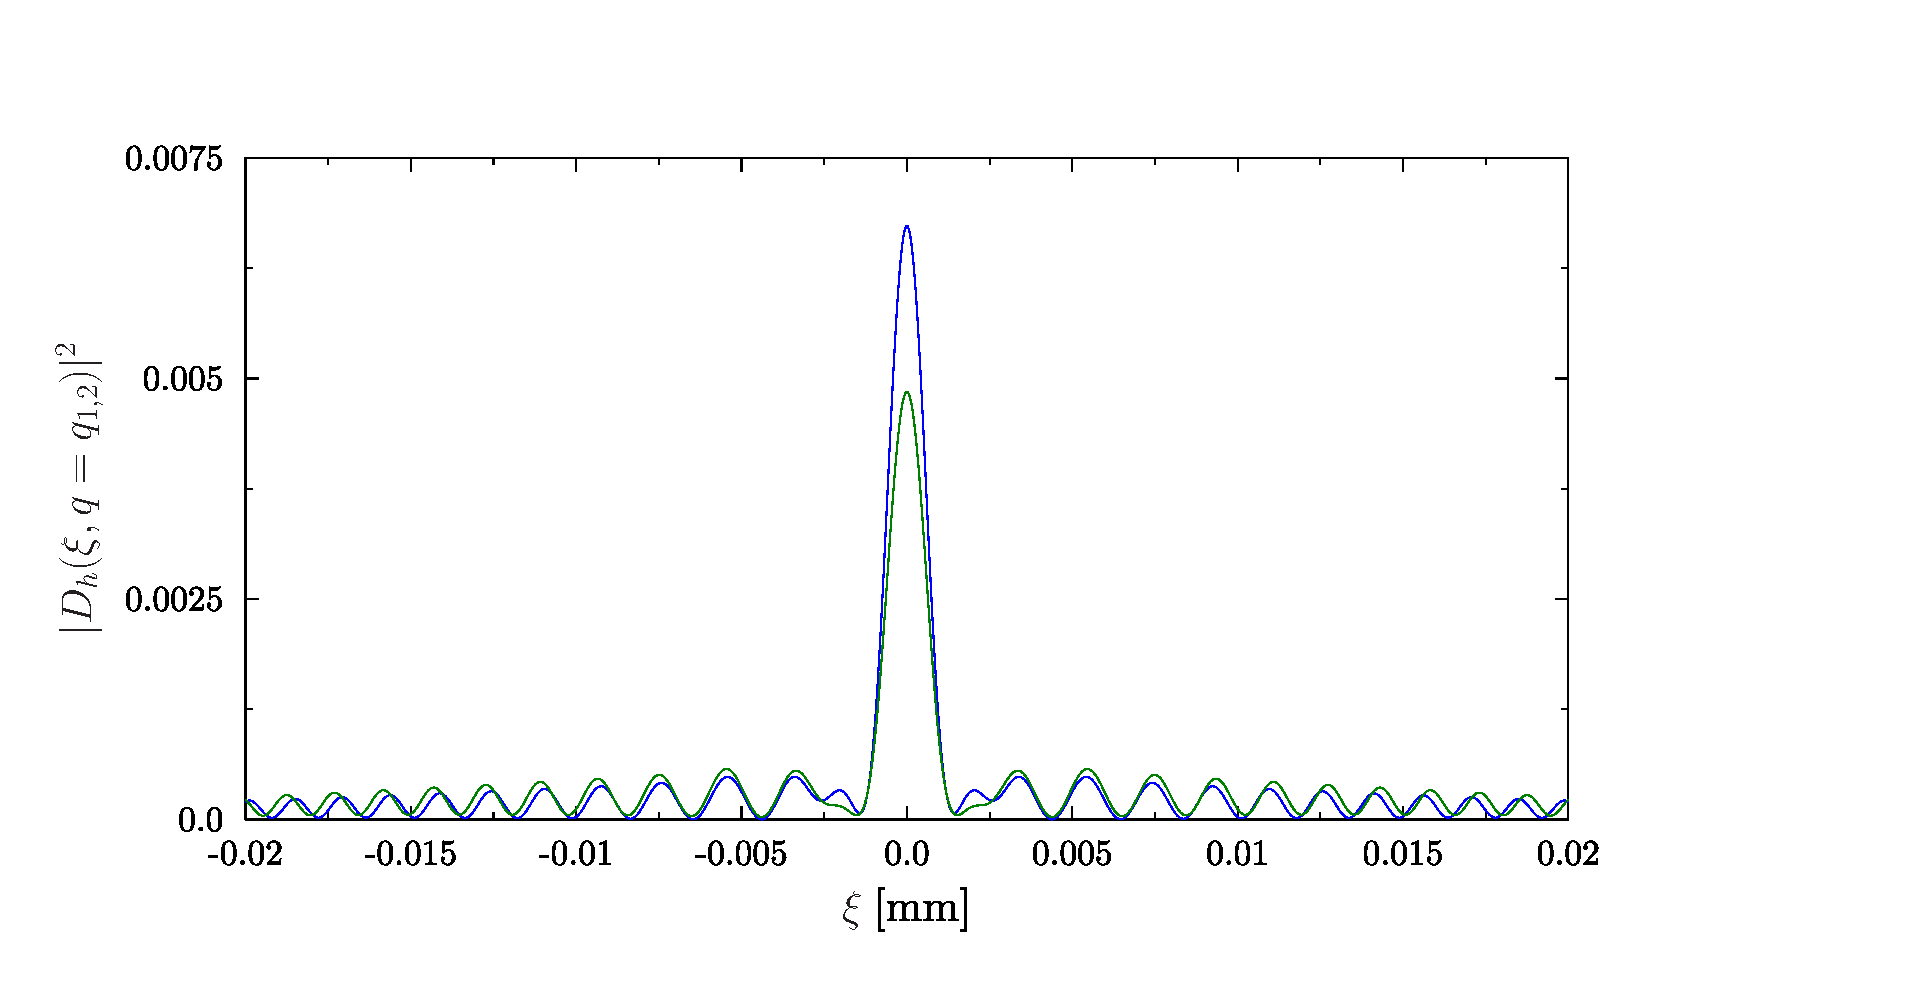
\includegraphics[width=0.46\textwidth]{bent1m17keV_profile.eps}}
\end{picture}

\end{figure}


%%%%%%%%%%%%%%%%%%%%%%%%%%%%%%%%  end put here figure %%%%%%%%%%%%%%%%%%%%%%%%%%%%%%%%%%%%%%%%%%%%%%%%

\end{document}